	\chapter{Ogólny opis projektu}
	Projekt powstał przy użyciu platformy FRAMES, w całości w języku programowania C++.\\
	
	Projekt dotyczy segmentacji ścian budynków w chmurze punktów 3D. Obliczone informacje zapisywane są do trzech warstw na wybranych etapach. Warstwa Horizontal Angles zawiera wartości kątów między wektorem normalnym najlepiej dopasowanej płaszczyzny a osią Z. Warstwa Smoothed Angles zawiera wygładzone wartości tych kątów. Ostatnia warstwa - Wall Index, zawiera odpowiednie indeksy wszystkich punktów. Indeksy te zostały podzielone na spełniające i niespełniające kryterium. Kryterium dotyczy wartości kątów - punkty o wartościach kątów powyżej ustalonego progu są kolejno numerowane, a te niespełniające kryterium otrzymują indeks 0. Dzięki temu, ustawiając wyświetlanie od wartości minimalnej 1, można dokładnie zobaczyć oddzielone obszary.\cite{pomerleau:hal-01178661} \\
	
	\begin{figure}[h!]%schemat wstawiania grafiki taki sam h! oznacza że wstaw w miejscu gdzie kod inaczej obras niesie w jakieś losowe miejsce(ogólnie wariuje z miejscem)
		\centering%wyśrodkowanie 
		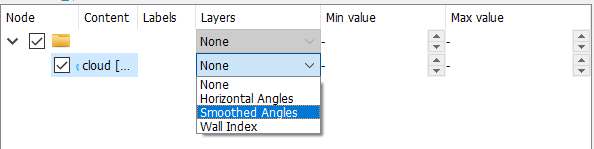
\includegraphics[width=\textwidth]{layers.png}%jaka wielkość obrazu i jaki obraz
		\caption{Warstwy}%podpis
		\label{fig:layers}%do referencji
	\end{figure}
	
	Jedyną wartością wprowadzaną do programu jest Neighbourhood radius, czyli promień sąsiedztwa wykorzystywany podczas segmentacji. Można jednak go nie wprowadzać, ponieważ domyślnie ustawiona jest wartość 7 i jest ona optymalna. \\

	\begin{figure}[h!]
		\centering
		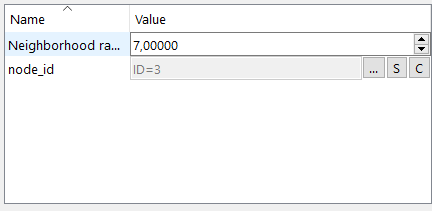
\includegraphics[width=0.5\textwidth]{input_values.png}
		\caption{Dane wejściowe}
		\label{fig:input}
	\end{figure}
	
	Program podczas wykonywania się, na bieżąco informuje użytkownika o postępie. Drukuje informację który algorytm z ilu jest aktualnie wykonywany, a gdy zostanie on wykonany, użytkownik zostaje o tym poinformowany. Dodatkowo dla każdego algorytmu powstał pasek postepu (progress bar).
	
	\begin{figure}[h!]
		\centering
		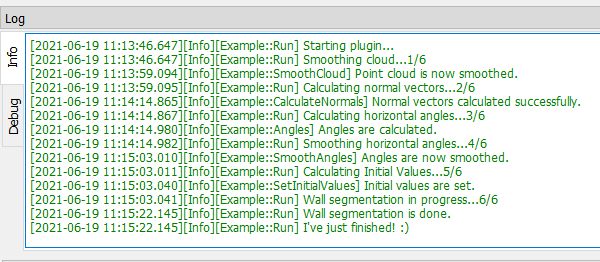
\includegraphics[width=\textwidth]{progress_info.png}
		\caption{Wyświetlanie informacji o postępie}
		\label{fig:progress_info}
	\end{figure}